\documentclass[12pt]{article}
\usepackage[utf8x]{inputenc}
\usepackage{amsmath}
\usepackage[switch]{lineno} 
\usepackage{graphicx}
\usepackage{color}
\usepackage{url}
\usepackage{subcaption}
\usepackage{tabularx}
\usepackage{booktabs}
\usepackage[margin=2.5cm]{geometry}
\usepackage{lineno}
\linenumbers

\usepackage{setspace}
\linespread{2}

\newcommand{\beginsupplement}{%
        \setcounter{table}{0}
        \renewcommand{\thetable}{S\arabic{table}}%
        \setcounter{figure}{0}
        \renewcommand{\thefigure}{S\arabic{figure}}%
     }

\title{Optimal strategies of Ecosystem Services provision \\for Amazonian production forests\\ {\small Running title: Ecosystem Services in Amazonian forests}}
\author{Camille Piponiot$^{1,2,3,4}$\footnote{Corresponding author: camille.piponiot@gmail.com}, Ervan Rutishauser$^{5,6}$, Géraldine Derroire$^{2}$, \\Francis E Putz$^{7}$, Plinio Sist$^{4}$, Thales A P West$^{7}$, Laurent Descroix$^{8}$,\\ Marcelino Carneiro Guedes$^{9}$ , Eur\'idice N. Honorio Coronado$^{10}$, \\Milton Kanashiro$^{11}$, Lucas Mazzei$^{11}$, Marcus Vinicio Neves d’Oliveira$^{12}$,\\ Marielos Peña-Claros$^{13}$, Ken Rodney$^{14}$, Ademir R Ruschel$^{11}$,\\ Cintia Rodrigues de Souza$^{15}$, Edson Vidal$^{16}$, \\Verginia Wortel$^{17}$, Bruno Hérault$^{4,18}$}
\date{}

\begin{document}

\maketitle 

\begin{enumerate}
\item  Université  de  Guyane,  UMR  EcoFoG  (Agroparistech,  CNRS,  Inra,  Université  des  Antilles,  Cirad), Kourou, French Guiana.
\item Cirad,  UMR  EcoFoG  (Agroparistech,  CNRS,  Inra,  Université  des  Antilles,  Université  de  Guyane), Kourou, French Guiana.
\item CNRS,  UMR  EcoFoG  (Agroparistech,  Inra,  Université des  Antilles,  Université  de  Guyane,  Cirad), Kourou, French Guiana.
\item Cirad, Univ Montpellier, UR Forests and Societies, Montpellier, France.
\item CarboForExpert, Hermance, Switzerland.
\item Smithsonian Tropical Research Institute, Balboa, Ancon 03092, Panama.
\item Department of Biology, University of Florida, Gainesville, United States.
%\item Instituto Boliviano de Investigación Forestal, Santa Cruz, Bolivia.
\item ONF-Guyane, Réserve de Montabo, F-97307 Cayenne, French Guiana.
\item Embrapa Amapá, Macapá, Brazil. 
\item Instituto de Investigaciones de la Amazonía Peruana, Iquitos, Peru.
\item Embrapa Amazônia Oriental, Belém, Brazil.
\item Embrapa Acre, Rio Branco, Brazil.
\item Forest Ecology and Forest Management Group, Wageningen University, Wageningen, Netherlands.
\item Iwokrama, Georgetown, Guyana
%\item Environmental Change Institute, University of Oxford, Oxford, United Kingdom
\item Embrapa Amazônia Ocidental, Manaus, Brazil.
\item Department of Forest Sciences, Luiz de Queiroz College of Agriculture, University of São Paulo, Piracicaba, Brazil.
\item Forest Management department, CELOS, Paramaribo, Surinam.
\item Institut National Polytechnique Félix Houphouët Boigny (INP-HB), Yamoussoukro, Côte d’Ivoire

\end{enumerate}


\section*{Abstract}

Although tropical forests harbour most of the terrestrial carbon and biological diversity on Earth they continue to be deforested or degraded at high rates. In Amazonia, the largest tropical forest on Earth, a sixth of the remaining natural forest is formally dedicated to timber production. Reconciling  timber production with the provision of other ecosystem services (ES) remains a major challenge for forest managers and policy-makers. This study applies a spatial optimisation of logging in Amazonian production forests to analyse potential trade-offs between timber production, carbon storage, and biodiversity conservation. Current logging regulations result in sub-optimal ES-use efficiency. Long-term timber provision would require the adoption of a land-sharing strategy that involves extensive low-intensity logging. By contrast, retention of carbon and diversity would be enhanced by a land-sparing strategy restricting high-intensive logging to designated areas such as the outer fringes of the region. Depending on management goals and societal demands, either choice will substantially influence the future of Amazonian forests. Overall, our results highlight the need for reevaluation of current logging regulations and regional cooperation among Amazonian countries to enhance coherent and trans-boundary forest management.

\vspace{1cm}
\textbf{Keywords} Amazonia; selective logging; multicriteria optimisation; ecosystem services; timber production; carbon; biodiversity

%\twocolumn

\section*{Introduction}

By storing about 30\% of the Earth’s terrestrial carbon \cite{Pan2013} and half of the world’s biodiversity \cite{Pimm2014}, regulating hydrological cycles \cite{Fisher2009a}, and furnishing a wide range of timber and non-timber goods, tropical forests are critical for human welfare and climate-change mitigation. These benefits notwithstanding, tropical forests are being converted into cropland at a higher-than-ever rate (1.1~Mkm$^2$ between 2000-2012 \cite{Hansen2013}) and are facing increasing pressure from other human activities \cite{Lewis2015}. One established way to counter tropical forest loss is to establish restricted access protected areas, but this simple dichotomy (protected or not) poorly reflects the wide gradient of forest uses and their effects (e.g., \cite{DeCastroSolar2015,Gibson2011}). 

In the tropics, nearly 40\% of the sawn wood traded annually is harvested from natural forests \cite{Payn2015}. Brazil is among the largest producers of tropical round wood, with 14 to 28 million m$^3$ (25-50\% of its total log production) annually harvested from Amazonian natural forests, mainly for local markets \cite{SFB2010,Santos2013,FAOstat2018}. Selective logging is the dominant harvesting system in the region, consisting in felling only a few commercial trees (5-10 trees ha$^{-1}$) in the forest. Because most of the forest cover remains after the harvest, selectively logged forests still maintain most of their initial carbon stocks, biodiversity, and other environmental services \cite{Putz2012}, and recovery of what is lost depends on logging practices, intensity, and the elapsed time before the next harvest \cite{Rutishauser2015,Piponiot2018}. For this reason, arguments are made for the integration of selectively logged forests into forest conservation schemes \cite{Edwards2014a}.  

Although recognition of the value of production forests in providing a diversity of ecosystem services (ES) is increasing, most conservation programs and payments for ES schemes focus on a single ES (e.g. carbon in REDD+ programs; \cite{Laing2016}) and therefore fail to account for the multi-functionality and complexity of forests \cite{VanderPlas2017}. Very few studies have addressed multi-criteria decision-making process regarding the optimisation of ES provision in tropical forests. For instance, a plot-level study in a logging concession in Suriname found that trade-offs between carbon stock conservation and timber recovery vary with logging intensity \cite{Roopsind2018}. Plot-level studies provide useful insights for local forest managers, but conservation-related policies need to be informed by broader-scale assessments that account for infrastructure planning, location of protected areas, and logging regulations \cite{Hein2006b}. Moreover, because ES provisioning varies across space (e.g. carbon stocks \cite{Avitabile2016} and biodiversity \cite{Jenkins2013}), complex spatial patterns in optimal ES provision are expected to emerge when plot-level information is scaled up \cite{Gibson2000}. Plot-level optimisation of ES provisioning can thus not be directly extrapolated to inform forest management policies at regional scales. Nevertheless, current logging regulations are typically based on results from local plot-level studies. For example, country-wide minimum cutting cycles (i.e. years between logging events) are set at 20 years in Bolivia and Peru, 25-35 years in Brazil, and 65 years in French Guiana \cite{Blaser2011}. There is thus a need to provide policymakers with regional assessments of ES trade-offs in Amazonian production forests.  

Here we explore optimal scenarios for ES provision in Amazonian production forests in a spatially-explicit framework. We analyse the effect of different logging intensities (i.e., no logging and logging at intensities of 10, 20, and 30 m$^3$ha$^{-1}$) and cutting cycles (15, 30, and 65 years) on post-logging timber recovery, carbon storage, and biodiversity conservation, which we refer to as ecosystem services (ES). Our main research questions are: (i) where, how much, and how often should timber harvest occur in order to optimise ES provision in Amazonian production forests; (ii) how do ES prioritisation and availability of production forest areas affect optimal logging configuration and resulting ES provision, and (iii) how projected changes in high-quality timber demand affect forest management and ES provision? 

We explore eight management strategies (Table~\ref{tab:strategies}) and identify the spatial logging configuration that optimises ES provision over the first cutting cycle, given a timber-production target of 30 Mm$^3$yr$^{-1}$, i.e., equivalent to timber production in the region \cite{Lentini2005}. Strategies differ in terms of (i) ES prioritisation, (ii) total forest area allocated to production, (iii) whether total timber stocks must fully recover (i.e., sustained timber yields), and (iv) whether a unique cutting cycle length is applied (30 years). We then compare the optimal spatial logging configurations and ES provisions associated with each strategy. Finally, we analyse the consequences of changing the timber-production target on ES provision.

\section*{Materials and methods}

\subsection*{Study region}

The study region is the Amazon region, located in tropical South America and straddling nine countries (Brazil, Bolivia, Colombia, Equator, French Guiana, Guyana, Peru, Suriname, and Venezuela). Amazonia is the most diverse and carbon-rich tropical biome on Earth \cite{Avitabile2016,Pimm2014} with around 600~Mha of tropical rainforest of which 400~Mha is considered “intact” (i.e., no detectable human impacts; \cite{Potapov2017}). To date, 36\% of Amazonian forests is under legal protection \cite{WDPA2016} (Figure~\ref{fig:pharv}). However since the 1970s and the opening of the Trans-Amazonian highway - the first highway built deep inside the forest - 20\% of the original forest extent has been replaced mainly by pastures and, more recently, soybean crops \cite{Kalamandeen2018,Fearnside2017}. Despite of the recent roads, a large portion of the forest biome is at a great distance from any road and thus inaccessible to most commercial activities (Figure~\ref{fig:pharv}).

Timber production through selective logging is the dominant forest use in the region \cite{Blaser2011}. About 15\% of Amazonian forests is designated for timber production \cite{FAO2011}. Estimates of annual sawlog production in these forests are around 30 Mm$^3$ \cite{Lentini2005}, even though the timber production in the Brazilian Amazon, the largest producer in the region, has been shown to decrease during the last decade due to a combination of the Brazilian government's fight against deforestation \cite{Nepstad2014} and the progressive substitution of tropical timber with other cheaper materials in construction \cite{Santos2013}. In Amazonia, logging intensities vary between 5-30~m$^3$ of timber extracted per ha, with an estimated average around 20~m$^3$ha$^{-1}$ in the Brazilian Amazon \cite{Asner2005}. Official minimum cutting cycle lengths vary among countries, from 20 years in Peru and Bolivia \cite{Fredericksen2003,Blaser2011}, to 65 years in French Guiana \cite{Gourlet-Fleury2004}. 

\begin{figure}
    \centering
    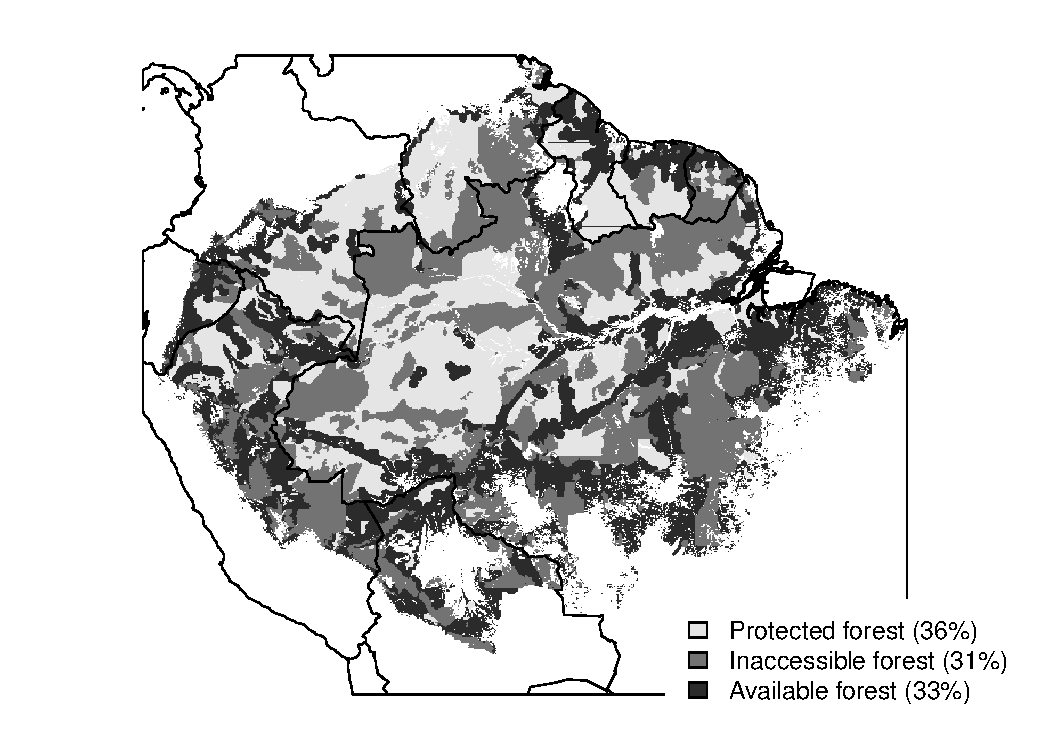
\includegraphics[width=\linewidth]{graphs/harv_areas_grey.pdf}
    \caption{Availability of Amazonian forests for logging (forest cover $>$ 90\%). Protected areas (light grey; does not include category VI of the IUCN) are not included in our analysis. Forests $>$ 25 km and $<$25 km from any road are depicted in dark and medium grey, respectively. Protected forests cover 210 Mha, inaccessible forests 176 Mha and accessible forests 190 Mha.}
    \label{fig:pharv}
\end{figure}

\subsection*{Optimisation framework}

The optimisation procedure finds the best spatial configuration of different logging strategies in Amazonia, which we divided into 556 1$^{\circ}$ cells (i.e., the coarsest resolution of input maps; see supplementary material~\ref{sec:defPPF}, Figure~\ref{fig:ppfDiagram}). The spatial optimisation seeks the most efficient spatial configuration of logging rules (cutting cycles and logging intensities) that minimises a cost function under pre-defined objectives. In the first step, an annual timber-production target is set (Figure~\ref{fig:basicDiagram}): the optimal solution must include enough harvested areas (i.e., cells in a raster map of the study region) to meet the target. In the second step, a management strategy is defined (see Table~\ref{tab:strategies} for a complete strategy description). The strategy includes (i) the weight of each ES (timber recovery, carbon storage and biodiversity conservation) in the cost function that will be minimised, (ii) the area of potential production forests (PPF), and (iii) some additional constraints: sustained timber yields (STY), unique cutting cycle length and intact forest landscape (IFL) conservation. The optimal spatial configuration for each strategy is then found using a methodology adapted from the optimisation software Marxan with Zones \cite{Watts2009}, using the package \textit{prioritzr} \cite{Hanson2018} developed in R programming language \cite{RCoreTeam2017}. Codes and data are available at \url{https://figshare.com/s/a60e3610337636a2b6ff}. 

\begin{figure}
    \centering
    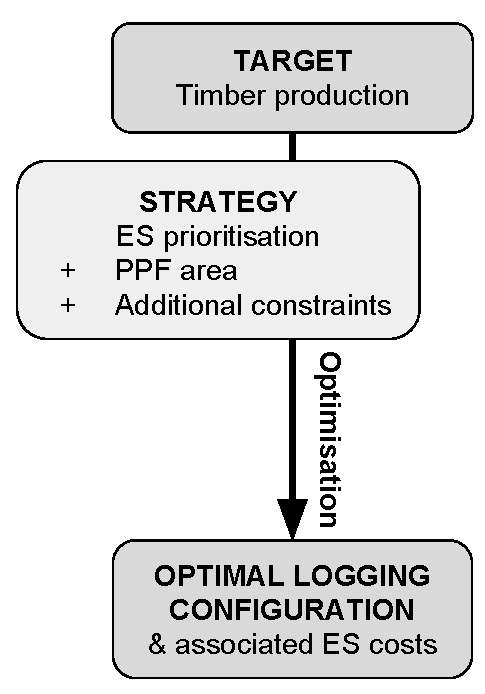
\includegraphics[width = 0.4\linewidth]{graphs/diagramSpatOptim}
    \caption{Spatial optimisation steps. Potential Production Forests (PPF) are all forests that are accessible and where logging is allowed. The eight strategies tested are summarised in Table~\ref{tab:strategies}. The resulting logging configuration and associated changes in ES provision with a timber harvest total of 30~Mm$^3$yr$^{-1}$ are presented in Figures~\ref{fig:mapsStrateg} and \ref{fig:scenESProv}, respectively. The effects of changing the timber-production target are presented in Figure~\ref{fig:incDemand}.}
    \label{fig:basicDiagram}
\end{figure}

\subsection*{Strategy description}

We tested different strategies to meet future timber demand in Amazonia (Table~\ref{tab:strategies}): (i) \textit{Timber}: only timber recovery is optimised to ensure long-term timber production, (ii) \textit{Carbon}: only carbon is optimised as a climate change mitigation strategy, (iii) \textit{Biodiversity}: only biodiversity is optimised as a conservation strategy, (iv) \textit{Balanced}: long-term timber provision, carbon and biodiversity conservation are balanced as a multi-functionality strategy, (v) \textit{Current}: balanced ES prioritisation under medium (30-year) cutting cycles, (vi) \textit{STY}: sustained timber yields (STY), i.e. the volume of timber extracted must be recovered at the end of the first cutting cycle, (vii) \textit{Road building}: all areas, except currently-protected areas, are made available for logging, and (viii) \textit{STY + Road building}: all areas, except currently-protected areas, are made available for STY logging. The annual timber-production target is first set to 30~Mm$^3$ (Figures~\ref{fig:mapsStrateg} and \ref{fig:scenESProv}); the effects of changing the timber-production target are then tested with targets between 10-80~Mm$^3$yr$^{-1}$ (Figure~\ref{fig:incDemand}). 

In scenarios (i-v), the area suitable for logging is the same as defined previously ("Currently accessible" in Table~\ref{tab:strategies}). In Road building scenarios (v-vi), we hypothesise that additional roads will be built: the new area suitable for logging ("All unprotected" in Table~\ref{tab:strategies}) corresponds to the total area with forest cover $>$90\% outside protected areas (independently of their current distance to a road), minus the 42\% corresponding to slopes and areas near rivers (see section~\ref{sec:ppf} and Figure~\ref{fig:ppfDiagram} in the supplementary material). 

\begin{table*}
    \centering
    \begin{tabularx}{\textwidth}{p{2cm} p{4.5cm} p{2cm} p{3.5cm} p{0.8cm} p{1cm}}
    \toprule
         Acronym & Strategy & ES prioritisation & PPF area &  STY & 30-yr cycle \\
         \midrule
         Timber & Long-term timber production & Timber  & Currently accessible & No & No\\
         Carbon & Climate change mitigation &  Carbon & Currently accessible & No & No\\
         Biodiversity & Biodiversity conservation &  Biodiversity & Currently accessible & No & No \\
         Balanced & Multi-functionality & Balanced & Currently accessible & No & No \\
         Current & Only 30-yr cutting cycles & Balanced & Currently accessible & No & Yes \\
         STY & Sustained timber yields & Balanced & Currently accessible & Yes & No \\
         Road building & Building roads to previously inaccessible areas & Balanced & All unprotected & No & No \\
         STY + Road building & Sustained timber yields with road building & Balanced & All unprotected & Yes & No \\
         \bottomrule
    \end{tabularx}
    \caption{Strategies tested in this study. ES prioritisation refers to the weights given to ESs in the optimisation process: either only one ES (timber, carbon or biodiversity) is optimised, or weights are balanced between timber production, carbon retention and biodiversity conservation. PPF are areas that can be logged in a given strategy: "Currently accessible" are areas that have $>$90\% forest cover, are not protected and are within 25~km of an existing road (Figure~\ref{fig:pharv}; "All unprotected" are areas with $>$90\% forest cover outside protected areas (no road-distance restriction): see Figure~\ref{fig:ppfDiagram} for maps of Amazonian PPF. Two optional constraints can be added: STY (Sustained Timber Yields) requires that the total timber stocks are recovered over all logged grid cells whereas the 30-year cycle constraint allows only 30-year cutting cycles.}
    \label{tab:strategies}
\end{table*}

\subsection*{ES prioritisation}

Spatially-explicit logging costs are estimated as the loss of each ES (i.e., carbon emissions, biodiversity loss, and decrease of the total forest timber stocks at the end of the cutting cycle) caused by logging operations and are calculated in each grid cell. To reflect the range of logging practices currently used in the region, logging is represented by one of the following: a logging intensity of 10 (Low), 20 (Medium) or 30 (High)~m$^3$ha$^{−1}$, and a cutting cycle length of 15 (Short), 30 (Medium) or 65 (Long) years, or no Logging. Medium intensity and cutting cycle length correspond to current median logging practices in Amazonia.

The total cost of allocating logging type $z$ to grid cell $p$ is estimated as: 

\begin{equation}
\begin{split}
    Cost_{p,z} = \alpha _T \cdot \frac{Prod_{p,z} - Rec_{p,z}}{\sum(vtot\cdot \omega_0)} + \alpha _C \cdot \frac{Cemi_{p,z}}{\sum (acs) }  + \alpha _B \cdot \frac{Rloss_{p,z}}{\sum (Rm + Ra)} 
\end{split}
\end{equation}

where $\alpha_T$, $\alpha_C$ and $\alpha_B$ are the relative weights of timber, carbon and biodiversity respectively. $Prod_{p,z}$ is the timber extracted in a grid cell $p$ when allocated to logging type $z$ and $Recp,z$ is the timber recovered at the end of the cutting cycle \cite{Piponiot2019}:  $Prod_{p,z}$ - $Rec_{p,z}$ is thus the net timber volume decrease after one cutting cycle. $Cemi_{p,z}$ represents the total carbon emissions caused by logging (yarding/skidding, road opening and incidental damage) minus the carbon recovered after logging \cite{Piponiot2016,Piponiot2016a}, integrated over the first cutting cycle. $Rloss_{p,z}$ represents vertebrates species loss (mammals and amphibians \cite{Jenkins2013}) by the end of the first cutting cycle in a grid cell $p$ when allocated to logging type $z$. Vertebrates and amphibians were chosen because of data availability (species richness maps and effect of selective logging on each taxa); moreover, they both play key roles in ecosystem functioning \cite{Wright2000,Fleming2009,Valencia-Aguilar2013}, and thus in provision of ESs.  
ES losses are standardised by their pre-logging ES value over all Amazon forests: $\sum(vtot\cdot \omega_0)$ is the total timber volume, $\sum (acs)$ is the total aboveground carbon stocks, and $\sum (Rm + Ra)$ is the sum of amphibians and mammals richness. ES costs are thus expressed as \% of their prelogging values. 
When a unique ES (timber, carbon or biodiversity) is prioritised in a given strategy, its weight is set to 1 and the others are set to 0. When ES prioritisation is balanced, $\alpha_T = \alpha_C = \alpha_B = \frac{1}{3}$.
To analyse the effect of ES prioritisation on final ES costs, we ran 66 simulations with all combinations of weights from 0 to 1, with 0.1 steps. Results are presented in the Supplementary material (Figure~\ref{fig:changeCosts}). 

\subsection*{Potential Production Forest area}
\label{sec:ppf}

In each grid cell, we considered only areas suitable for logging, referred to as "potential production forests" (PPF). The area of all unprotected PPF was estimated as areas (i) having at least 90\% of forest cover \cite{Hansen2013}, and (ii) not being under a full protection status \cite{WDPA2016}. To estimate the currently accessible PPF area, the areas that are more than 25~km away from any road were removed; a road is here defined as any motorable track registered in OpenStreetMap \cite{OSM2018}. Additional information is provided in the Supplementary material (Section~\ref{sec:defPPF}). 
The total areas of PPF ("all unprotected" and "currently available") are then calculated for each grid cell. Because only 50-80\% of a production forest area is considered suitable for logging due to steep slopes, riparian buffers and previous heavy degradation \cite{Feldpausch2006,Verissimo2002}, the total area of PPF was multiplied by a coefficient $\pi = 58\%$, calibrated with data from French Guiana concessions \cite{Piponiot2019}.

\subsection*{Additional constraints}

\subsubsection*{Sustainable timber yields}

An optional sustainable timber yields (STY) constraint was added to the \textit{STY} and \textit{STY + Road building} strategies. In these strategies, timber recovery over all grid cells must be greater or equal to harvested timber volumes: 

\begin{equation}
    \sum_{p}\sum_{z} (Rec_{p,z} - Prod_{p,z}) \geq 0 
\end{equation}
where $Prod_{p,z}$ and $Rec_{p,z}$ area respectively the harvested and recovered timber in grid cell $p$ allocated to logging type $z$.

\subsubsection*{Unique cutting cycle length}

In the \textit{Current} strategy, grid cells can be allocated to only four logging types: 30-year cutting cycles (Medium) with 10-, 20- or 30-m$^3$ha$^{-1}$ logging intensities, or no logging. 

\subsubsection*{IFL conservation}

Finally, an additional constraint to conserve biodiversity is added to all strategies that consists of conserving intact forest landscapes (IFLs) defined as forests with no detectable sign of human activity \cite{Potapov2017}. IFLs are irreplaceable for biodiversity conservation \cite{Gibson2011}, especially for species that are highly sensitive to forest degradation. Because Amazonian forests have high levels of endemism and all regions are not equivalent in terms of species composition, we defined the biodiversity conservation objective as follow: in each of the six ecoregions (according to Ter Steege et al. \cite{TerSteege2013}), namely the Guiana Shield, eastern Amazon, southeastern Amazon, central Amazon, southwestern Amazon, and northwestern Amazon, at least 80\% of IFLs are to remain unlogged. Those include forests in protected areas, inaccessible forests ($>$25 km from a road or track), or forests inside grid cells allocated to the "No Logging" type. 


\section*{Results}

\subsection*{Optimal logging configuration under a 30~Mm$^3$yr$^{-1}$ timber-production target}

Our predictions when timber production is optimised (i.e. \textit{Timber} strategy) result in exploitation of 88\% of all production forests over one cutting cycle, of which 7\% are under high-intensity short-cycle logging, 3\% under low-intensity short-cycle logging and 78\% under low-intensity long-cycle logging (Figure~\ref{fig:mapsStrateg}a). In contrast, maximising carbon and biodiversity retention results in the preservation of 85\% of available forests, and logging 15\% of available forests under the highest intensity (30~m$^3$ha$^{-1}$) and shortest cutting cycle (15 years) allowed (Figure~\ref{fig:mapsStrateg}b-c). Logged areas are distributed around outer fringes of Amazonia: southeastern Amazonia for both carbon and biodiversity, northern Amazonia for carbon and the southwestern border for biodiversity. 

Balancing timber, carbon and biodiversity (i.e. \textit{Balanced} strategy) results in preservation of 74\% of available forests, logging 13\% of available forests under high-intensity (30~m$^3$ha$^{-1}$) short-cycle (15 years) logging and 13\% under low-intensity (10~m$^3$ha$^{-1}$) long-cycle (65 years) logging (Figure~\ref{fig:mapsStrateg}d). Similar to the \textit{Carbon} and \textit{Biodiversity} strategies, heavily logged areas are concentrated on the peripheries of the Basin, especially on its southeastern border and low-intensity logging is concentrated in the south and northwest whereas central, western and northeastern Amazonia remain mostly unlogged. Allowing only 30-year cutting cycles (\textit{Current} strategy) results in the preservation of a smaller share of available forests (48\%) while 16\% are logged under high intensity (30~m$^3$ha$^{-1}$) and 36\% under low intensity (10~m$^3$ha$^{-1}$;  Figure~\ref{fig:mapsStrateg}e). 

Constraining the full recovery of the timber volume extracted at the end of the cutting cycle (STY; Figure~\ref{fig:mapsStrateg}f) results in allocating a higher proportion of forests to low-intensity long-cycle logging (29\% versus 13\% in the \textit{Balanced} strategy) and preserving fewer areas (60\% versus 70\% in the \textit{Balanced} strategy).

Increasing forest accessibility through road building (Figure~\ref{fig:mapsStrateg}g) results in a spatial configuration similar to the \textit{Balanced} strategy. The total area under high-intensity (30~m$^3$ha$^{-1}$) short-cycle (15 years) logging is slightly lower than in the \textit{Balanced} strategy (13~Mha instead of 14~Mha) and the total area under low-intensity (10~m$^3$ha$^{-1}$) long-cycle (65 years) logging is higher (24~Mha instead of 14~Mha). Adding a STY constraint (\textit{STY + Road building} strategy) increases the proportion of low-intensity long-cycle logging (15\% versus 12\% in the \textit{Road building} strategy) and decreases the proportion of preserved areas (79\% versus 82\% in the \textit{Road building} strategy)  (Figure~\ref{fig:mapsStrateg}h). 


\begin{figure*}
    \centering
    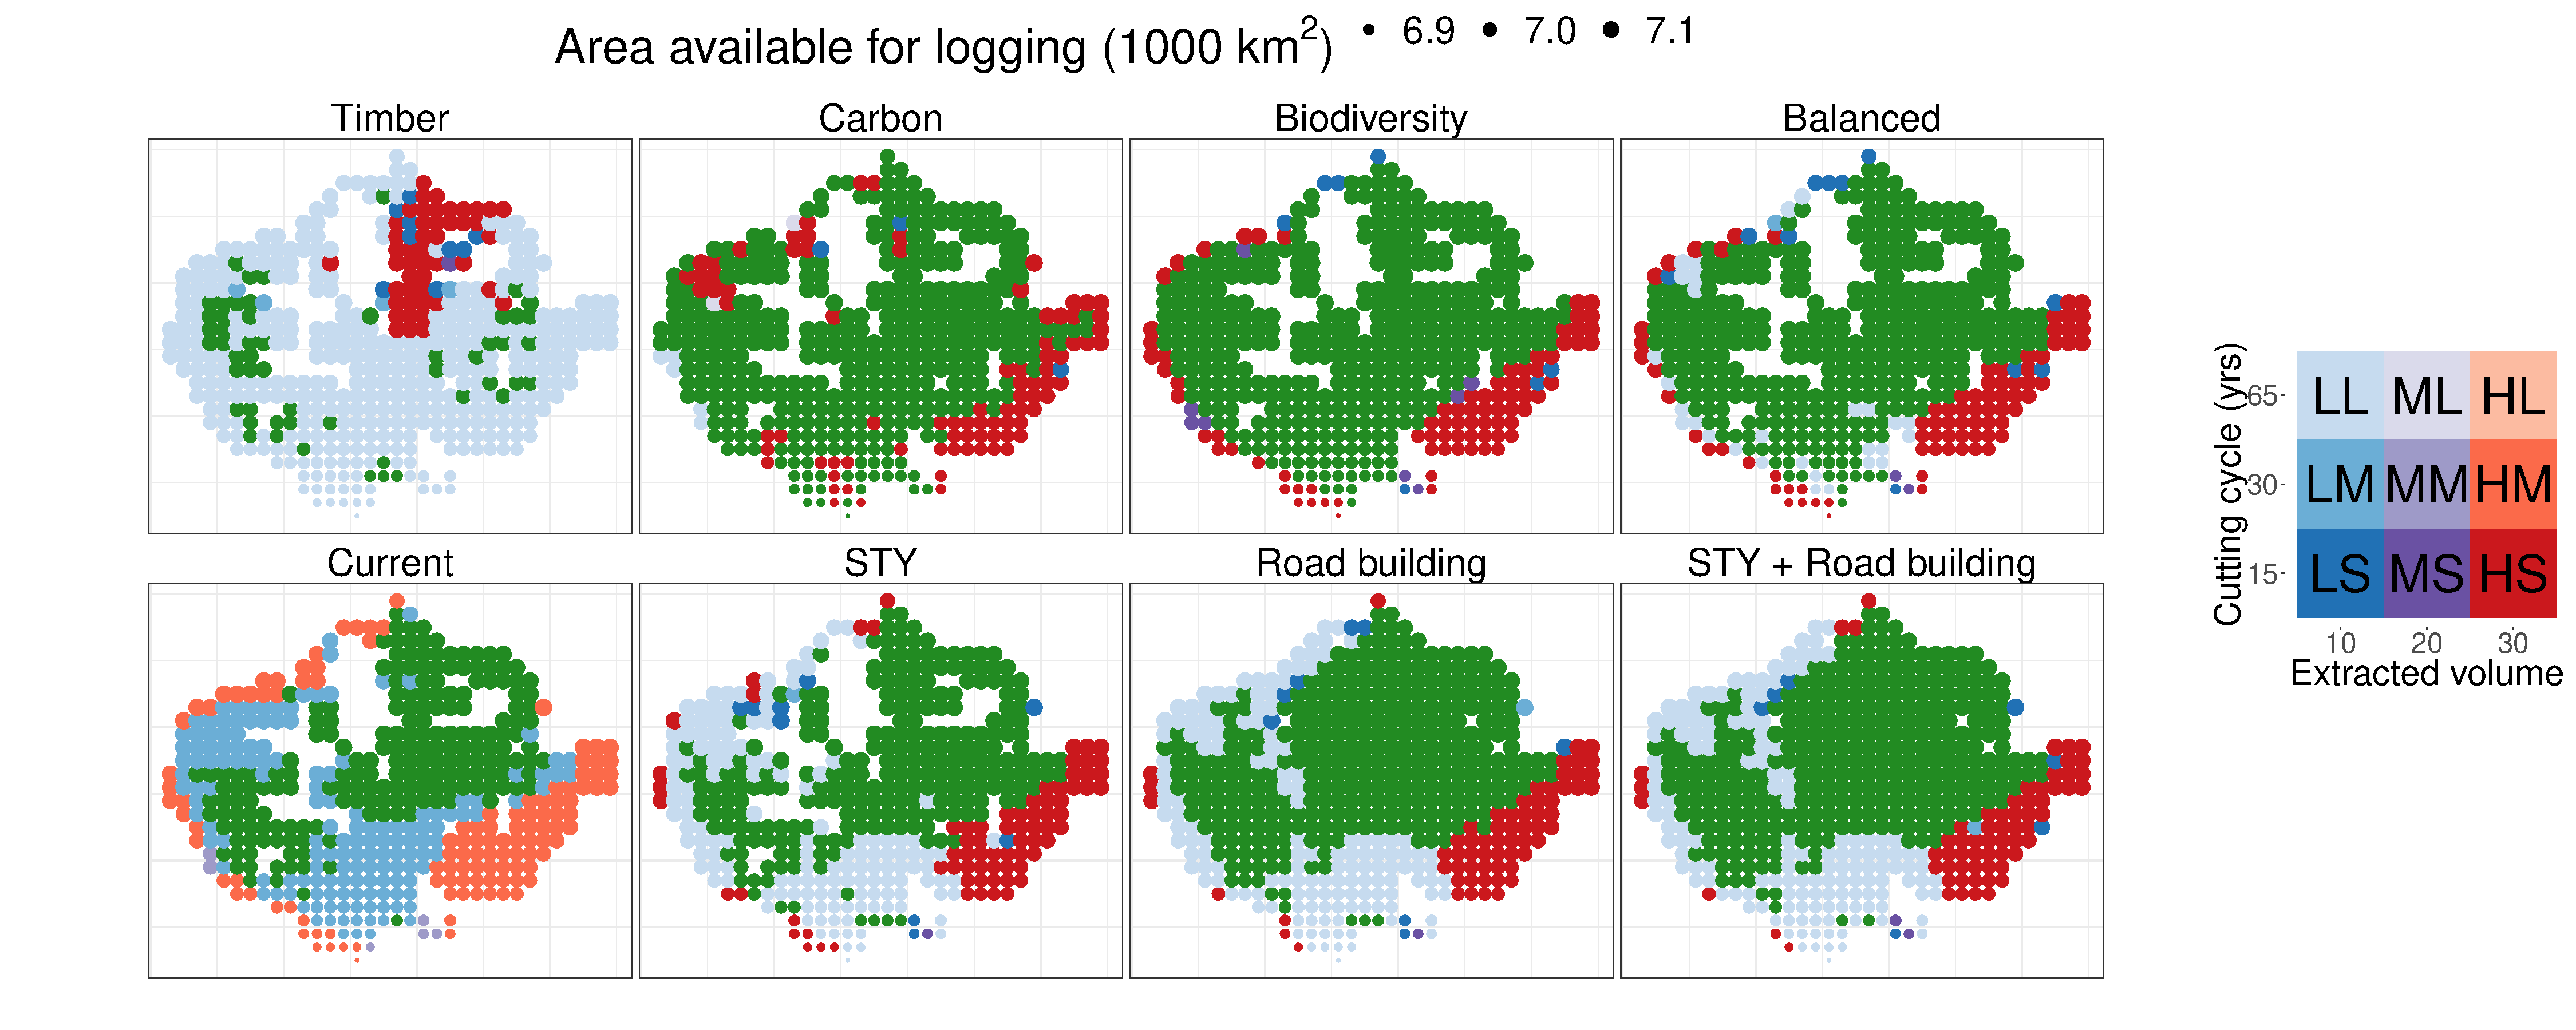
\includegraphics[width=0.8\linewidth]{graphs/mapsScenarios.pdf}
    \caption{Results of spatial optimisation with the eight strategies defined in Table~\ref{tab:strategies} with a natural forest timber production target of 30~Mm$^3$yr$^{-1}$. Green areas are not logged, white areas are not in PPF. The size of each dot is proportional to the PPF area (total area available for logging). Logging type colour (blue - purple - red) represent the logging intensity (Light: 10, Medium: 20 and High: 30~m$^3$ha$^{-1}$). The logging type transparency represents the cutting cycle length (Short: 15, Medium: 30, Long: 65 years): light colours correspond to longer cycles.}
    \label{fig:mapsStrateg}
\end{figure*}

\subsection*{Effect of strategy choice on ES provision}

The \textit{Timber} strategy results in the best final timber stocks (+2.3\% of initial timber stocks, Figure~\ref{fig:scenESProv}a), the lowest carbon stocks (-4\% of initial carbon stocks, Figure~\ref{fig:scenESProv}b) and the least biodiversity retention (-6.4\% of initial value, Figure~\ref{fig:scenESProv}c). The \textit{Carbon}, \textit{Biodiversity}, \textit{Balanced} and \textit{Road building} strategies result in timber losses (-2.1\%, -2.1\%, -1.1\% and -0.3\%, respectively), but low carbon emissions (-1.4\%, -1.6\%, and -1.7\%, and -1.3\%, respectively) and low diversity losses (-2.3\%, -1.9\%, -2.5\%, and -2.2\%, respectively). The strategies with a STY constraint (\textit{STY} and \textit{STY + Road Building}) result in no variation in timber stocks (Figure~\ref{fig:scenESProv}a), at the cost of higher carbon and biodiversity losses than the strategies without the STY constraint (the \textit{Balanced} and \textit{Road building} strategy, respectively; Figure~\ref{fig:scenESProv}b-c). In contrast, the \textit{Current} strategy performs very poorly at provision of all three ESs. Indeed, this strategy results in the highest reduction of timber stocks (-2.1\%) and the second highest reduction of carbon stocks (-3.3\%) and biodiversity (-4.4\%), not far behind the \textit{Timber} strategy. 

\subsection*{Changing the timber production target}

Our model framework allowed to test the ability of the eight forest management strategies to satisfy timber demands that range from 10 to 80 Mm$^3$yr$^{-1}$. Increasing timber production results in an increase of area harvested (except for the \textit{Timber} strategy; Figure~\ref{fig:incDemand}a), and a reduction of ES provision (Figure~\ref{fig:incDemand}d-f). For the \textit{Timber} strategy, the total area logged is already at its maximum value (around 80~Mha) even with low timber production targets (Figure~\ref{fig:incDemand}a). For this strategy, increasing timber production from 20 to 80~Mm$^3$yr$^{-1}$ would result in increasing mean logging intensity by 60\% (from 10 to 16~m$^3$ha$^{-1}$) and decreasing mean cutting cycle length by 15 years (from 60 to 45 years) (Figure~\ref{fig:incDemand}b-c).

The \textit{Carbon} and \textit{Biodiversity} strategies have similar behaviours: both rely upon high-intensity (30~m$^3$ha$^{-1}$) short-cycle (15 years) logging, independently from the timber production target (Figure~\ref{fig:incDemand}b-c). Increasing timber production in both strategies results in a linear increase in logged areas (Figure~\ref{fig:incDemand}a).

When ES prioritisation is balanced (Balanced and Road building strategies), timber production is mostly achieved through low-intensity long-cycle logging when the production target is low (Figure~\ref{fig:incDemand}b-c). However, increasing timber production under both strategies generates a shift from low-intensity long-cycle logging to high-intensity short-cycle logging (Figure~\ref{fig:incDemand}b-c; Figure~\ref{fig:mapsIncDemand}), and extended total area logged.

Adding the STY constraint to the \textit{Balanced} and \textit{Road building} strategies (respectively the \textit{STY} and \textit{STY + Road building} strategies) does not drastically change simulations when production targets are low ($<$~20~Mm$^3$yr$^{-1}$). At higher production targets, mean logging intensity plateaus at approximately 15~m$^3$ha$^{-1}$ and the mean cutting cycle stabilises at 50 years, resulting in a sharp increase in the total area logged (Figure~\ref{fig:incDemand}a). The STY constraint can only meet 50~Mm$^3$yr$^{-1}$ in currently available PPF (i.e. in the \textit{STY} strategy) and 60~Mm$^3$yr$^{-1}$ including all PPF (i.e. in the \textit{STY + Road building} strategy).

Finally, the \textit{Current} strategy (i.e. balanced ES prioritisation with cutting cycles of 30 years) results in low-intensity logging when the total production remains lower than 20~Mm$^3$yr$^{-1}$ (Figure~\ref{fig:incDemand}b). Increasing timber production results in a sharp increase in both the total area logged and the logging intensity (Figure~\ref{fig:incDemand}a-b). When the timber production target reaches 80~Mm$^3$yr$^{-1}$, the total area logged is close to its maximum value (around 80~Mha; Figure~\ref{fig:incDemand}a) and all areas logged are under high-intensity logging (30~Mm$^3$yr$^{-1}$; Figure~\ref{fig:incDemand}b). In terms of ES provision, the \textit{Current} strategy performs poorly compared to others, especially at high timber-production target (Figure~\ref{fig:incDemand}d-f).

\begin{figure*}
    \centering
    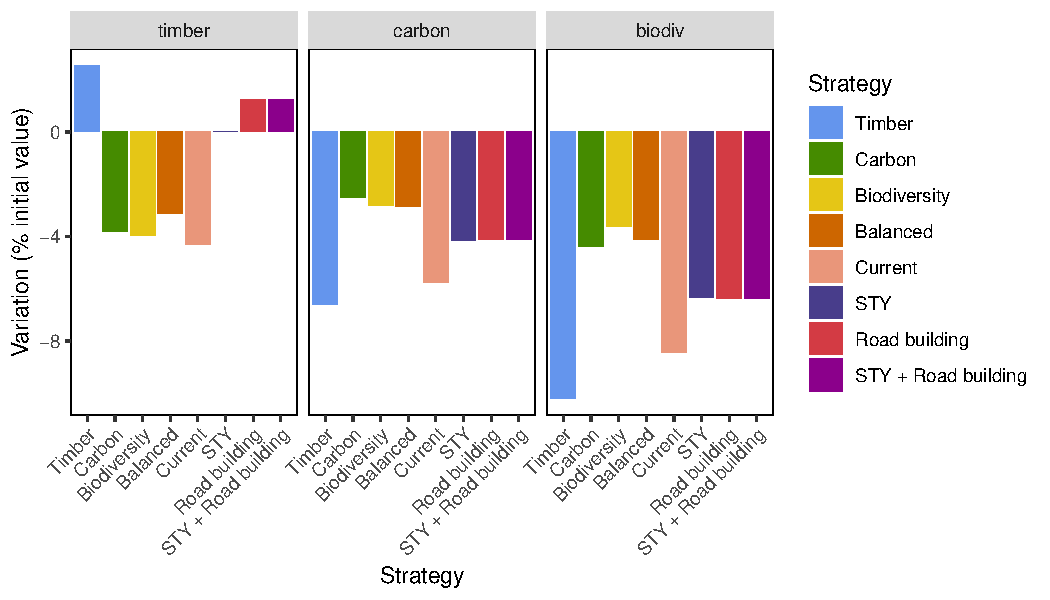
\includegraphics[width=\linewidth]{graphs/costsScenario}
    \caption{Impact of the eight management strategies (described in Table~\ref{tab:strategies}) in terms of total ES provision (\% of the initial ES value) with the timber production target of 30~Mm$^3$yr$^{-1}$. (a) Variation of regional timber stocks; (b) variation of regional carbon stocks; and, (c) variation of regional biodiversity. A positive value indicates an increase in total ES provision; a negative value indicates a loss in total ES provision. Variation of ES provision are standardised by the initial value of a given ES (i.e. initial timber, carbon stocks and mammals and amphibians richness for biodiversity) over all areas with forest cover $>$90\% (see Figure~\ref{fig:ppfDiagram}: "All forests"). 
 }
    \label{fig:scenESProv}
\end{figure*}

\begin{figure*}
    \centering
    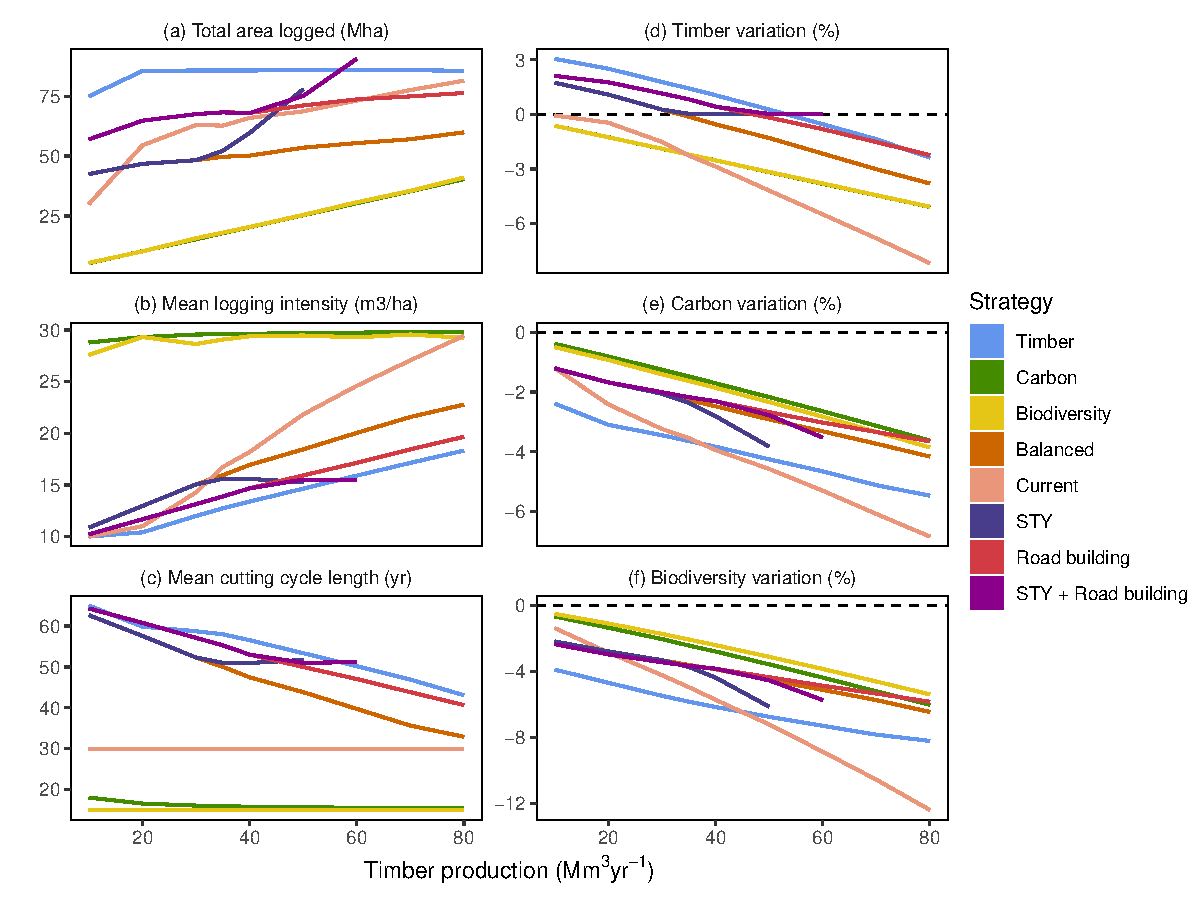
\includegraphics[width=\linewidth]{graphs/increasingDemand.pdf}
    \caption{ Characterisation of different strategies for timber production with different timber production targets. (a) Total area logged (Mha). (b) Mean logging intensity in logged areas (m$^3$ha$^{-1}$). (c) Mean cutting cycle length (yr). (d) Variation of timber stocks (\% of the initial value). (e) Carbon emissions (\% of the initial value) (f) Variation of biodiversity value (\% of the initial value). The eight strategies' characteristics are summarised in Table~\ref{tab:strategies}. \textit{STY} and \textit{STY + Road building} strategies cannot sustainably provide more than 50 and 60 Mm$^3$ of annual timber production respectively. In plots (d-f), values are calculated over all areas outside of protected areas. Additional maps with distribution of logging types (intensity, cutting cycle) are provided in the supplementary material (Figure~\ref{fig:mapsIncDemand}).
}
    \label{fig:incDemand}
\end{figure*}

\section*{Discussion}

\subsection*{Optimisation of ES provision in Amazonian managed forests}

Our results show that regional optimisation of ES provision results in a strong spatial structuring of logging. Intermediate logging cycles (30 years) and intensities (20~m$^3$ha$^{-1}$) are virtually never chosen, and imposing some standardisation (e.g. 30-year cutting cycles in the \textit{Current} strategy) results in sub-optimal ES provision. This spatial heterogeneity in our results provides evidence that forest management could benefit from regional studies, instead of applying uniform logging regulations based on a small set of local studies. Therefore, the optimisation approach applied in this study has many implications for sustainable forest management in Amazonia. 

Ecosystem service provision by selectively logged forests is relatively well studied, but the ESs are often treated one or two at a time, that limits insights in the trade-offs. Trade-offs between carbon retention and timber recovery were found, at the plot scale, in Guiana's logged forests \cite{Roopsind2018}, and between timber production and species richness across the tropics \cite{Burivalova2014}. These trade-offs were also shown to depend on land tenure and deforestation risk \cite{Griscom2018}. Forest owners generally manage forests to maximise financial benefits, through timber or non-timber forest products harvesting, eco-tourism or payments for ecosystem services. Local studies can help forest owners set locally-relevant conservation goals, but generally fail to account for regional objectives.

Climate change mitigation and nature conservation goals are intrinsically trans-boundary, and are better addressed at regional or global scales \cite{Hein2006}. For instance, efficient delimitation of protected areas, definition of logging rules and road planning should be developed at regional scale among countries. Informing decision-makers with large-scale multi-criteria analyses will thus be key to develop evidence-based policies. Today, very few studies have assessed regional-scale ESs trade-offs in Amazonia (but see \cite{OConnell2018}) and, despite its importance for the regional economy, none has investigated timber production and associated regional-scale ESs trade-offs.

\subsection*{Regional differences in Amazonian forests and consequences for ES provision}
            	
The spatial configuration of optimal logging (Figure~\ref{fig:mapsStrateg}) is closely linked to major regional differences in the functioning of Amazonian forests. Forests of the Guiana Shield (northeastern Amazonia) grow on nutrient poor soils and suffer few natural disturbances \cite{Espirito-Santo2014}, which selected for low turnover rates and slow-growing species \cite{Grau2017}. Guiana shield forests thus harbour large amounts of carbon \cite{Avitabile2016} and support rich vertebrate communities \cite{Denis2018} due to their long-term persistence \cite{Barthe2017} and are therefore, not selected for logging when biodiversity and carbon are optimised (Figure~\ref{fig:mapsStrateg}a-b). Forests of the Guiana Shield have also been shown to play a crucial role in the Amazonian hydrological cycle \cite{Bovolo2018,Staal2018}, enhancing the importance of their conservation in future management strategies. Similarly, northern and central Amazonian forests encompass high diversity of vertebrates \cite{Jenkins2013} and carbon \cite{Avitabile2016}, and are thus rarely selected for logging when biodiversity and carbon storage are prioritised (Figure~\ref{fig:mapsStrateg}a-b). If conservation is the main objective of Amazonian forest management, the consolidation of the protected area network in central and northeastern Amazonian forests will provide high benefits for conservation and climate change mitigation, especially if this promotes a higher connectivity between existing protected areas \cite{Hansen2007}. Southeastern forests have, in turn, relatively lower diversity and carbon stocks. They are thus often allocated to high-intensity short-cycle logging when carbon and biodiversity are optimised (Figure~\ref{fig:mapsStrateg}a-b). However, due to intense forest degradation through logging, fragmentation and/or wildfire \cite{Davidson2012,Foley2007}, timber production in southeastern PPF may have been overestimated, even in closed-canopy forests \cite{Asner2004}. Southeastern forests are also predicted to experience longer and more severe droughts in the near future \cite{Duffy2015}, with potential negative impacts on timber provision in the region.  
 
\subsection*{Land-use strategies, trade-offs and implications for policy-making}

Current logging regulations (e.g. 35-year maximum cutting cycle in the Brazilian Amazon) were thought to be a compromise between producing enough timber to make financial benefits, and letting the forest recover long enough to make logging sustainable \cite{Seydack2012}. Several studies have shown that these logging rules are not sufficient to recover pre-logging forest characteristics \cite{Sist2007,Zimmerman2012,Piponiot2018}. Moreover, our results show that current regulations (e.g. imposing 30-year cutting cycles, similar to the \textit{Current} strategy), increase the loss of all ESs and leads to sub-optimal management (Figure~\ref{fig:scenESProv}). The standard strategy often promoted for the maintenance of timber production in tropical forests is to change national regulations so that cutting cycles are longer and logging intensities are lighter, but these recommendations may result in a significant increase in total harvested forest areas to compensate for the reduction in timber extracted per ha and per year.

Our results reveal that, in fact, the main trade-off is between long-term provision of timber, and conservation of carbon stocks and biodiversity (Figure~\ref{fig:changeCosts}). These results fit into the broader "land sharing vs land sparing" debate, and whether timber production should concentrate on a few intensely-logged areas (land sparing), or be carried at low intensity over the entire landscape (land sharing). Land-sparing logging was shown to create heterogeneous landscapes that favour higher levels of beta-diversity and maintenance of biodiversity at landscape scale \cite{DeCastroSolar2015,Edwards2014}. It has been argued that under strong forest governance, land-sharing logging could optimise both carbon and diversity retention \cite{Griscom2018}. More recently, a simulation exploring different management strategies in East Kalimantan forests found that the optimal forest conservation strategy consisted in mixing both approaches: intensifying timber production through the conversion of degraded forests into plantations, and implementing reduced-impact logging in current logging concessions and some natural forests \cite{Runting2018}. Our findings also show that a land-sparing approach (e.g. the \textit{Carbon} and \textit{Biodiversity} strategies) not only minimises biodiversity loss (Figure~\ref{fig:mapsStrateg}b, Figure~\ref{fig:incDemand}f), but also reduces carbon emissions (Figure~\ref{fig:mapsStrateg}a, Figure~\ref{fig:incDemand}e). However, these land-sparing strategies result in low timber recovery compared to a land-sharing strategy (e.g. the \textit{Timber} strategy, Figure~\ref{fig:scenESProv}a).

There is therefore no win-win strategy to sustain current timber demand and ESs provision in production forests. Further, current application of intermediate logging rules increases ESs losses (Figure~\ref{fig:incDemand}d-f). The fate of Amazonian production forests hence depends on political choices and on future societal demand for ESs. If maintaining long-term timber supplies from natural production forests is the goal \cite{Zarin2007}, then low-intensity logging should be preferred and applied across most of the Amazon, notably in the western part of the Basin (Figure~\ref{fig:mapsStrateg}a). In contrast, if society demands preservation of carbon and biodiversity (e.g. carbon-based policies like REDD+ \cite{Stickler2009}), policies should focus on conserving intact inland forests while allowing high-intensity logging on the fringes of the Amazon Basin. High-intensity logging will probably result in a sharp decrease of timber resources in over-harvested areas. Alternative pathways include active forest restoration with intensive silviculture and mixed-species timber plantations \cite{Lamb2005} to stimulate production in over-harvested forests, but such interventions may require to adopt policies and financial incentives to compensate for additional costs, e.g. through payments for ecosystem services \cite{Salzman2018}, and to secure land tenure \cite{Smith2006}.

Increasing the PPF area (in the \textit{Road building} strategies, Table~\ref{tab:strategies}) provides more options for optimising logging spatial configuration, and hence tends to increase ES provision overall: the \textit{Road building}  and \textit{STY  + Road building} strategies have higher ES values than the \textit{Balanced} and \textit{STY} strategies, respectively (Figure~\ref{fig:incDemand}d-f). Nevertheless, insofar as logging roads render forests vulnerable to hunting, wood-fuel harvesting and illegal logging \cite{Laurance2009a}, uncontrolled forest degradation in new PPF areas could increase the environmental costs of the \textit{Road building} strategy.
 
\subsection*{How to further improve ES provision in production forests?}

Standardising logging rules (e.g. applying a unique 30-year cutting cycle in the \textit{Current} strategy) resulted in the lowest ES provision in our results: improving forest management will thus require some adaptation to local ecological specificities, e.g. forest types, recovery rates or local patterns of biodiversity. Applying such detailed regulations will require highly-trained technicians to define, licence and implement forest management plans. Additionally, silvicultural treatments such as liana-cutting \cite{Mills2019}, thinning and girdling \cite{Pena-Claros2008}, or enrichment planting \cite{Schwartz2013,Navarro-Cerrillo2011}, can also significantly increase timber recovery with reasonable financial costs (e.g. \cite{Mills2019}). Some treatments, such as  girdling of non-commercial trees, may however imply trade-offs with carbon retention \cite{Roopsind2018}, and biodiversity conservation \cite{Ruslandi2017}. 

We did not explore the potential of improved logging techniques, generally known as Reduced-Impact Logging (RIL), to enhance simultaneously both ESs and timber production. A compelling body of evidence shows that RIL practices could provide large improvements in terms of timber recovery, carbon emissions and biodiversity protection \cite{Griscom2019,Putz2008c,Tobler2018,West2014}, and many authors thus argue that they should be an essential point in forest management strategies \cite{Griscom2018,Runting2018}. Despite this evidence, RIL technique remained poorly implemented in the field \cite{Ellis2019}. We therefore decided to base our study on currently dominant logging practices, keeping in mind that ES provision would be improved if RIL was more widely implemented.

One key point to bear in mind is that our simulations are restricted to the first cutting cycle. This is particularly important for STY strategy, as even if our predictions ensure a sustainable timber production over the first cutting cycle, we cannot rule out decreases afterwards. There is almost no data on multi-cycle logging in Amazonia, and most permanent forest plots have only been logged once \cite{Sist2015}, although most PPF may have undergone multiple illegal re-entries \cite{Tritsch2016a}. Gathering more information on the effect of multiple cutting cycles on forest dynamics is of utmost importance to glimpse at the future of production forests.

Finally, even though our findings provide an interesting insight on potential trade-offs that future forest managers and decision-makers will face, a large part (20-60\%) of logging is illegal in the Amazon \cite{Brancalion2018,Finer2014}. Changing logging rules to maintain the environmental value of production forests can be jeopardised by lack of control over their application. Improving Amazonian forests' governance will be key to maintain ecosystem services through informed management. 


%Optimising ESs in production forests at the Amazon-basin scale results in strong spatial structuring of optimal logging configuration, a finding that could not be derived from only local studies. Depending on ES priorities, optimal logging configurations range from timber-oriented land-sharing that promote low-intensity logging and result in sub-optimal biodiversity and carbon retention, to conservation-oriented land-sparing strategies that maximise forest diversity and carbon retention but results in rapid timber depletion and will thus require alternative timber sources in the future. Our results stress the need for a concerted re-evaluation of current logging rules in Amazonia, and the consequences of current management choices for ES provisioning in future production forests.


\section{Acknowledgements}

This study was partially funded by the GFclim project (FEDER 20142020, Project GY0006894), two Investissement d’Avenir grants of the ANR: CEBA (ANR-10-LABEX-0025), and the REsilience of Managed Amazonian FORests project funded by LabEx Agropolis (ANR-10-LABX-0001), and Embrapa. The study was carried out in the framework of the Tropical managed Forests Observatory (TmFO), supported by the Sentinel Landscape program of CGIAR (Consultative Group on International Agricultural Research) Forest Tree and Agroforestry Research Program. We thank all TmFO members who contributed data and participated to the discussions related to this paper, and especially the Instituto Boliviano de Investigaci\'on Forestal.

\section{Author contributions}
CP and BH designed the study, CP performed simulations and wrote the first draft, CP, ER, FEP, TAPW and BH wrote the paper, all other authors contributed data, commented on and approved the manuscript.

\clearpage

\bibliographystyle{nature}
\bibliography{biblio}


\onecolumn
\beginsupplement
\appendix
\begin{center}
    { \huge \textbf{Supplementary material}}
\end{center} 

\section{Quantifying the effect of logging on ESs}
\label{sec:ESestimation}

\subsection{Timber production and recovery}

From a previously developed volume recovery model calibrated at the Amazonian scale \cite{Piponiot2019}, we extracted: (i) the total volume $vtot_p$ (m$^3$ha$^{-1}$) in grid cell $p$, (ii) the proportion of potentially commercial timber $\omega 0_p$ and (iii) the potential timber recovery $vrec_{p,z}$ at the end of a cutting cycle $trot_z$ and after a logging intensity $vext_z$ ($z$ being the logging type). All parameters were set to their maximum likelihood value.

The mean annual timber production over the first cutting cycle in grid cell $p$ in logging type $z$ is equal to: 
\begin{equation}
\label{eq:prod}
    Prod_{p,z}  =  \frac{min\big(vext_z, (vtot_p\cdot \omega 0_p) \big) \cdot area_p}{trot_z}
\end{equation}

where $vext_z$ is the extracted volume in logging type $z$, $vtot_p\cdot \omega 0_p$ is the potential timber volume (the actual extracted volume cannot exceed the potential timber volume), $area_p$ is the area available for logging and $trot_z$ is the cutting cycle length.

The mean annual timber recovery over the first cutting cycle in grid cell $p$ in logging type $z$ is equal to: 

\begin{equation}
\label{eq:rec}
    Rec_{p,z} = \frac{vrec_{p,z}\cdot area_p}{trot_{p,z}}
\end{equation}

\subsection{Carbon emissions}

The effect of logging on carbon emissions is here quantified as the mean difference to the initial carbon stock over the cutting cycle. It was assessed as the difference of two terms: (i) the initial carbon loss caused by logging, (ii) minus the carbon storage from forest regrowth, averaged over the cutting cycle. 

The initial carbon loss caused by logging is threefold: (i) from extracted logs; (ii) from road building (deforestation), (iii) from incidental damage during logging operations \cite{Piponiot2016}. 

The carbon emissions from extracted logs in grid cell $p$ under logging type $z$ was assessed as: 

\begin{equation}
\label{eq:cext}
    Cext_{p,z} = Prod_{p,z} \cdot WDext_p \cdot  area_p
\end{equation}

with $Prod_{p,z}$ the actual logging intensity (in m$^3$ha$^{-1}$), $area_p$ is the area available for logging (ha) in grid cell $p$ and $WDext_p$ is the mean wood density of commercial trees in grid cell $p$ (see supplementary section~\ref{supmat:wdext} for wood density estimation). 

The carbon emissions from road building were estimated as follow: 

\begin{equation}
\label{eq:croad}
    Cdefor_{p,z} = Pdefor \cdot acs_p \cdot area_p
\end{equation}

where $Pdefor = 4.7 $\% is the estimated proportion of a logged area that is deforested for infrastructure (roads, logging decks and main skid trails) according to Piponiot et al. \cite{Piponiot2016} and $acs_p$ is the mean aboveground carbon density (MgC.ha$^{-1}$) in grid cell $p$, extracted from a global carbon map \cite{Avitabile2016}. 

Carbon losses from damaged trees were assessed as follows: 

\begin{equation}
\label{eq:cdam}
    Cdam_{p,z} = \frac{acs_p  - Prod_{p,z} \cdot WDext_p } {1 + \left(\frac{acs_p}{Prod_{p,z} \cdot WDext_p}  -1 \right)^\theta} \cdot area_p
\end{equation}

with $\theta$ a parameter of the model: the model justification and calibration are presented in supplementary section~\ref{supmat:cdam}. 

Post-logging carbon recovery $Crec_{p,z}$ was assessed with the methodology developed by Piponiot et al. \cite{Piponiot2016a}.  
All parameters were set to their maximum likelihood value. 

For each grid cell $p$ and each logging type $z$, the mean annual carbon emissions from grid cell $p$ under logging type $z$ are thus calculated as: 

\begin{equation}
\label{eq:cemi}
    Cemi_{p,z} = Cext_{p,z} + Cdefor_{p,z} + Cdam_{p,z} -  \sum_{t=1}^{trot_z} \frac{Crec_{t,p,z}}{trot_z} 
\end{equation}

\subsection{Biodiversity}

We chose to model the effect of logging on amphibians and mammals richness because they are key animals in forest ecosystems: amphibians are good indicators of global ecosystem health \cite{Welsh1998,Collins2003} and mammals ensure many ecosystem functions, among which pollination \cite{Fleming2009} and seed dispersal \cite{Wright2000,Muscarella2007}. We used global maps of mammals and amphibians richness derived from IUCN species range maps \cite{Jenkins2013,MapBiodiv}, which can fairly represent patterns of conservation priority \cite{Marechaux2017}.

The impact of logging on mammals and amphibians was assessed with the equation: 

\begin{equation}
\label{eq:rloss}
Rloss_{p,z} = \left(Rm_{p} \cdot \beta m + Ra_{p} \cdot \beta a  \right)  \cdot vext_z \cdot area_p 
\end{equation}

where $Rloss_{p,z}$ is the loss of vertebrate richness (mammals and amphibians) in grid cell $p$ and logging type $z$, $Rm_{p}$ and $Ra_p$ are the pre-logging richness of mammals and amphibians respectively \cite{Jenkins2013}, $\beta m = 1.44$ and $\beta a = 1.53$  are the estimated slopes of post-logging species loss in the Neotropics for mammals and amphibians respectively, according to Burivalova et al. \cite{Burivalova2014}. $vext_z$ is the logging intensity in logging type $z$.
We hypothesize that amphibians and mammals richness do not recover after logging (no effect of cutting cycle length). 

\subsection{Wood density estimation}
\label{supmat:wdext}

\begin{figure*}
    \centering
    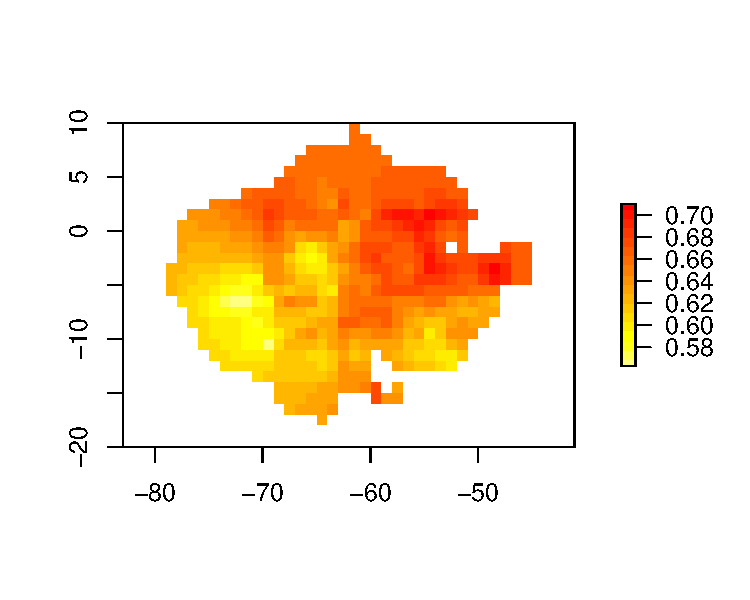
\includegraphics[width=0.7\linewidth]{graphs/map_WDext.pdf}
    \caption{Map of predicted wood density from interpolation of RadamBrasil data}
    \label{sfig:wdext}
\end{figure*}

We used 2646 1-ha forest inventory plots spanned over the Brazilian Amazon from the RadamBrasil project \cite{Radam2017}, in which all trees $\geq$33 cm diameter at breast height (DBH) were measured, identified to the species level and had their volume estimated. 

In every plot we estimated the mean wood density of all commercial stems (as defined in a previous study \cite{Piponiot2019}) with the R package BIOMASS \cite{Rejou-Mechain2017}.
Values were then interpolated with the R package \textit{automap} \cite{gstat} on a 1$^{\circ}$ resolution grid (Supplementary figure~\ref{sfig:wdext}).


\subsection{Carbon damage model}
\label{supmat:cdam}

\begin{figure}
    \centering
    \begin{subfigure}[b]{0.3\textwidth}
        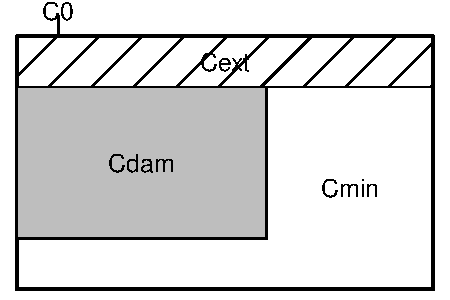
\includegraphics[width=\linewidth]{graphs/schemaDam.pdf}
        \caption{Diagram of carbon pools in the damage model.}\label{fig:schemaDam}
    \end{subfigure}
    ~ 
    \begin{subfigure}[b]{0.55\textwidth}
    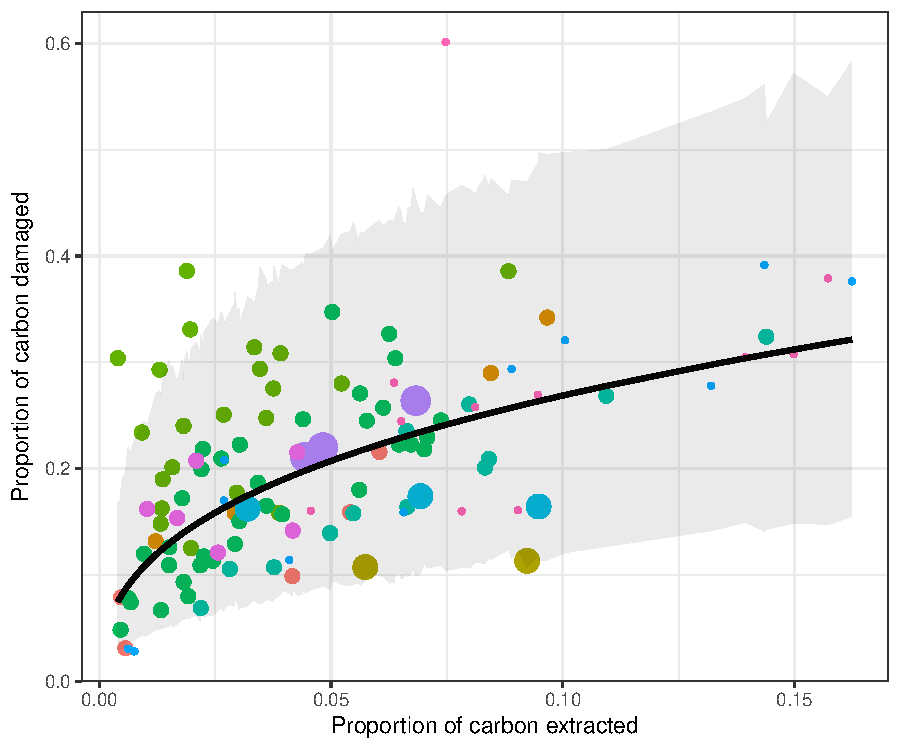
\includegraphics[width=\linewidth]{graphs/damModel.pdf}
    \caption{Carbon damage model. Coloured dots are data from one plot, with each colour representing one site and the size of the dot being proportional to the plot's size. The black line is the maximum likelihood prediction, and the shaded area is the 95\% confidence interval.}\label{fig:damModel}
    \end{subfigure}
\end{figure}

To estimate carbon emissions from logging damage we calibrated a model with data from 115 plots (129.25~ha total) in 11 experimentally logged sites spread in Amazonia \cite{Sist2015}. In all plots the identity of harvested trees was recorded, and at least one pre-logging and two post-logging forest inventories were carried out. In each forest inventory the diameter at breast height (DBH) of all stems $>$~20 cm DBH were measured, and trees were identified to the lowest taxonomic level (83\% species, 16\% genus, 2\% not identified). 
From forest inventories the above ground carbon and wood density of all trees $>$ 20 cm DBH  were estimated with the R package BIOMASS \cite{Rejou-Mechain2017}. 

The carbon extracted from plot $j$ was estimated as: 

\begin{equation}
    Cext_j = \sum_{i} \underbrace{a_j \cdot DBH_i^b}_{\text{volume of tree $i$}} \cdot WD_i
\end{equation}

with $DBH_i$ is the DBH of the logged tree $i$, $WD_i$ is its wood density and $a_j$, $b$ are the two parameters of a volumetric equation calibrated at the Amazonian scale \cite{Piponiot2019}. 

The carbon of damage was estimated as: 

\begin{equation}
    Cdam_j = C0_j - Cext_j - Cmin_j
\end{equation}

where $C0_j$ is the pre-logging above ground carbon of all trees $>$ 20 cm DBH in plot $j$, and $Cmin_j$ is the minimum above ground carbon during the four years following logging operations (Figure~\ref{fig:schemaDam}). 

We define the following variables: 

\begin{itemize}
    \item $RatioExt_j=\frac{Cext_j}{C0_j}$ is the proportion of the initial above-ground carbon $C0_j$ that is extracted of the plot $j$; 
    \item $RatioDam_j = \frac{Cdam_j}{C0_j-Cext_j}$ is the proportion of damage in the carbon left in plot $j$ after logging operations. 
\end{itemize}

We calibrated the following model (see Figure~\ref{fig:damModel}): 

\begin{equation}
logit(RatioDam_j) \sim \mathcal{N}(\theta \cdot logit(RatioExt_j), \sigma_D^2)
\end{equation} 

with $\theta$ the slope of the relationship, and $\sigma_D$ the standard deviation. 


\clearpage

\section{Mapping potential production forest areas}

\label{sec:defPPF}

To define the area of potential production forests, we first assessed the total forest area ("All forests" in Figure~\ref{fig:ppfDiagram}) as the area with forest cover $>$ 90\% in each 1~$^{\circ}$ grid cell, using a map of forest cover by Hansen and colleagues with a 4~km resolution \cite{Hansen2013}. The area was then multiplied by a factor $\pi = 58\%$, corresponding to the typical proportion of harvestable areas in a forest concession (excluding slopes, riparian reserves, etc), calibrated with data from French Guiana concessions \cite{Piponiot2019}. 
We then assessed the area of unprotected forests ("All unprotected" in Figure~\ref{fig:ppfDiagram}) as the area with forest cover $>$ 90\% (4~km resolution map) excluding all pixels inside strictly protected areas (categories I-V of the IUCN) as defined in the World Database on Protected Areas \cite{WDPA2016}. The area was then multiplied by a factor $\pi = 58\%$. 
We finally assessed the area of unprotected forests close to ("Currently accessible" in Figure~\ref{fig:ppfDiagram}) as all unprotected 4-km pixels with forest cover $>$ 90\% that are $<$ 25 km from any motorable track recorded in OpenStreetMap \cite{OSM2018}. The area was then multiplied by a factor $\pi = 58\%$. 

\begin{figure}
    \centering
    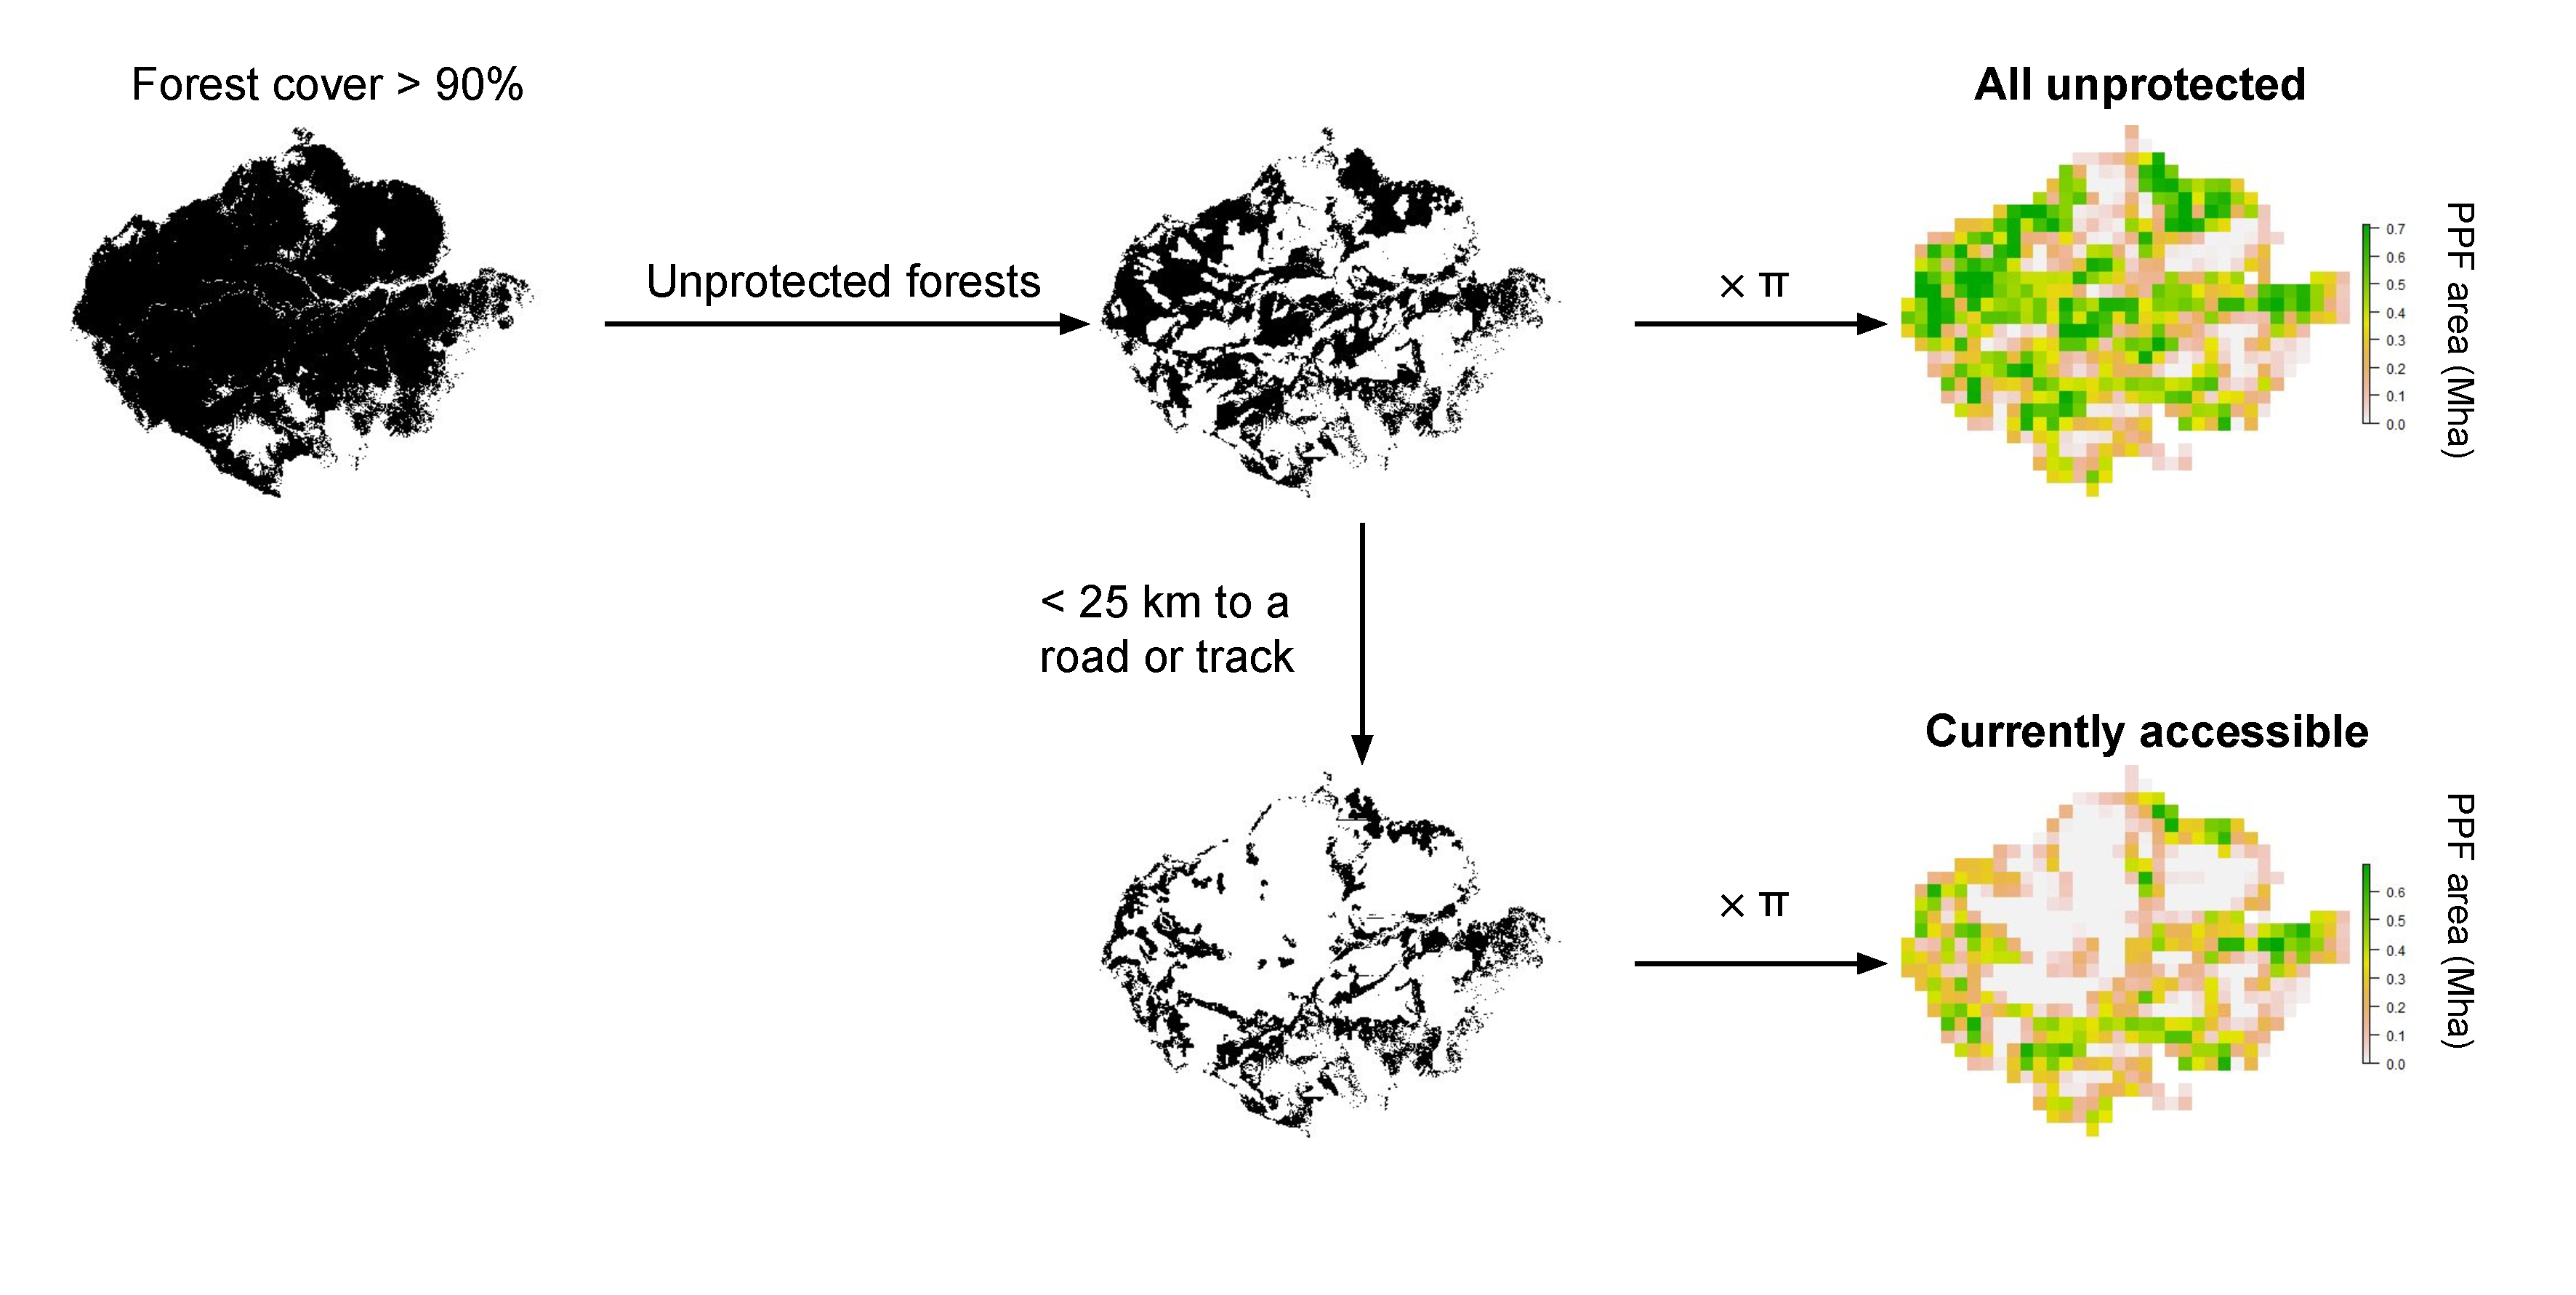
\includegraphics[width=\linewidth]{graphs/PPFareaDiagram.pdf}
    \caption{Flowchart of the estimation of potential production forests (PPF) area in each cell of the 1$^{\circ}$ grid of Amazonia. Input 4-km-resolution rasters are (i) the forest cover from Hansen et al. \cite{Hansen2013}, (ii) the protected area network from the IUCN \cite{WDPA2016} and (iii) the map of all motorable roads and tracks from the Open Street Map \cite{OSM2018}. $\pi = 0.58$ is the proportion of harvestable areas in forest concessions (based on data from French Guiana). }
    \label{fig:ppfDiagram}
\end{figure}

\clearpage


\begin{figure*}
    \centering
    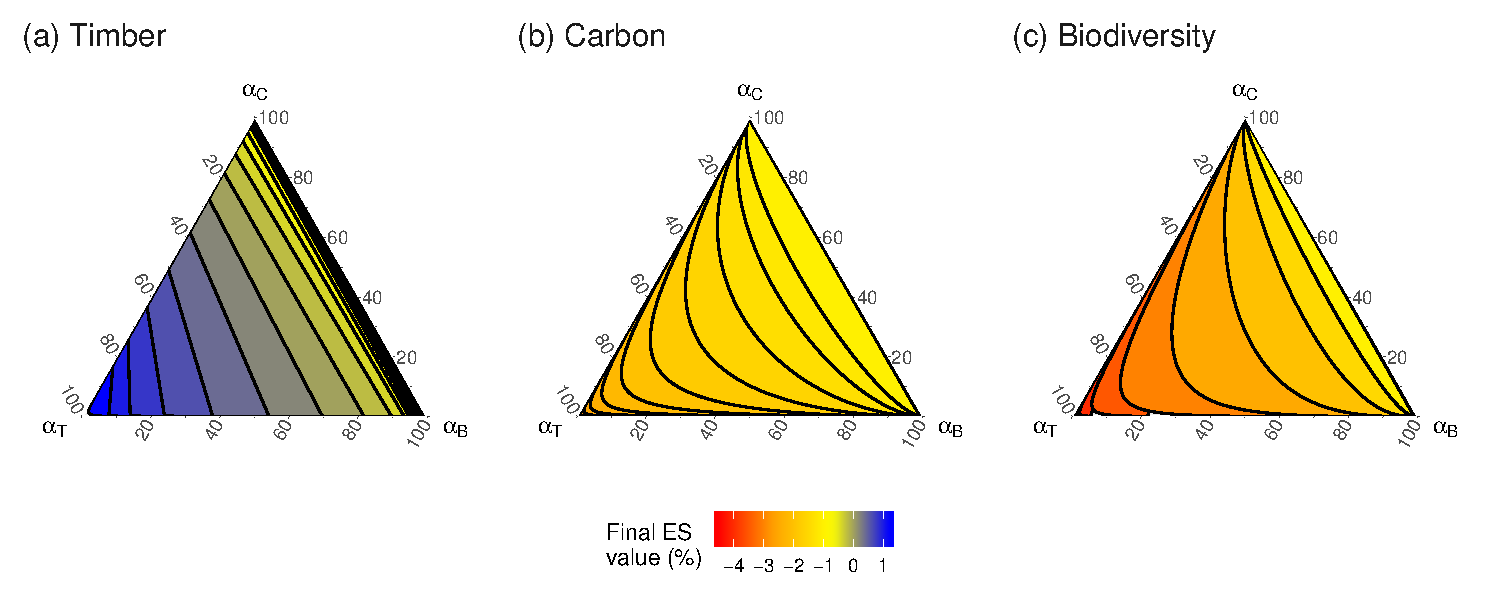
\includegraphics[width=\textwidth]{graphs/changingESweights.pdf}
    \caption{ES variation depending on the weight given to each ES in the optimisation process. $\alpha_T$, $\alpha_C$ and $\alpha_B$ are the weights given to timber, carbon and biodiversity, respectively (as a percentage of the total weight). Each ES variation is expressed as a proportion (\%) of the initial value for the corresponding ES. For example a carbon variation of -2\% means that total carbon emissions associated to logging correspond to 2\% of initial carbon stocks.} 
    \label{fig:changeCosts}
\end{figure*}


\clearpage

\begin{figure*}
    \centering
    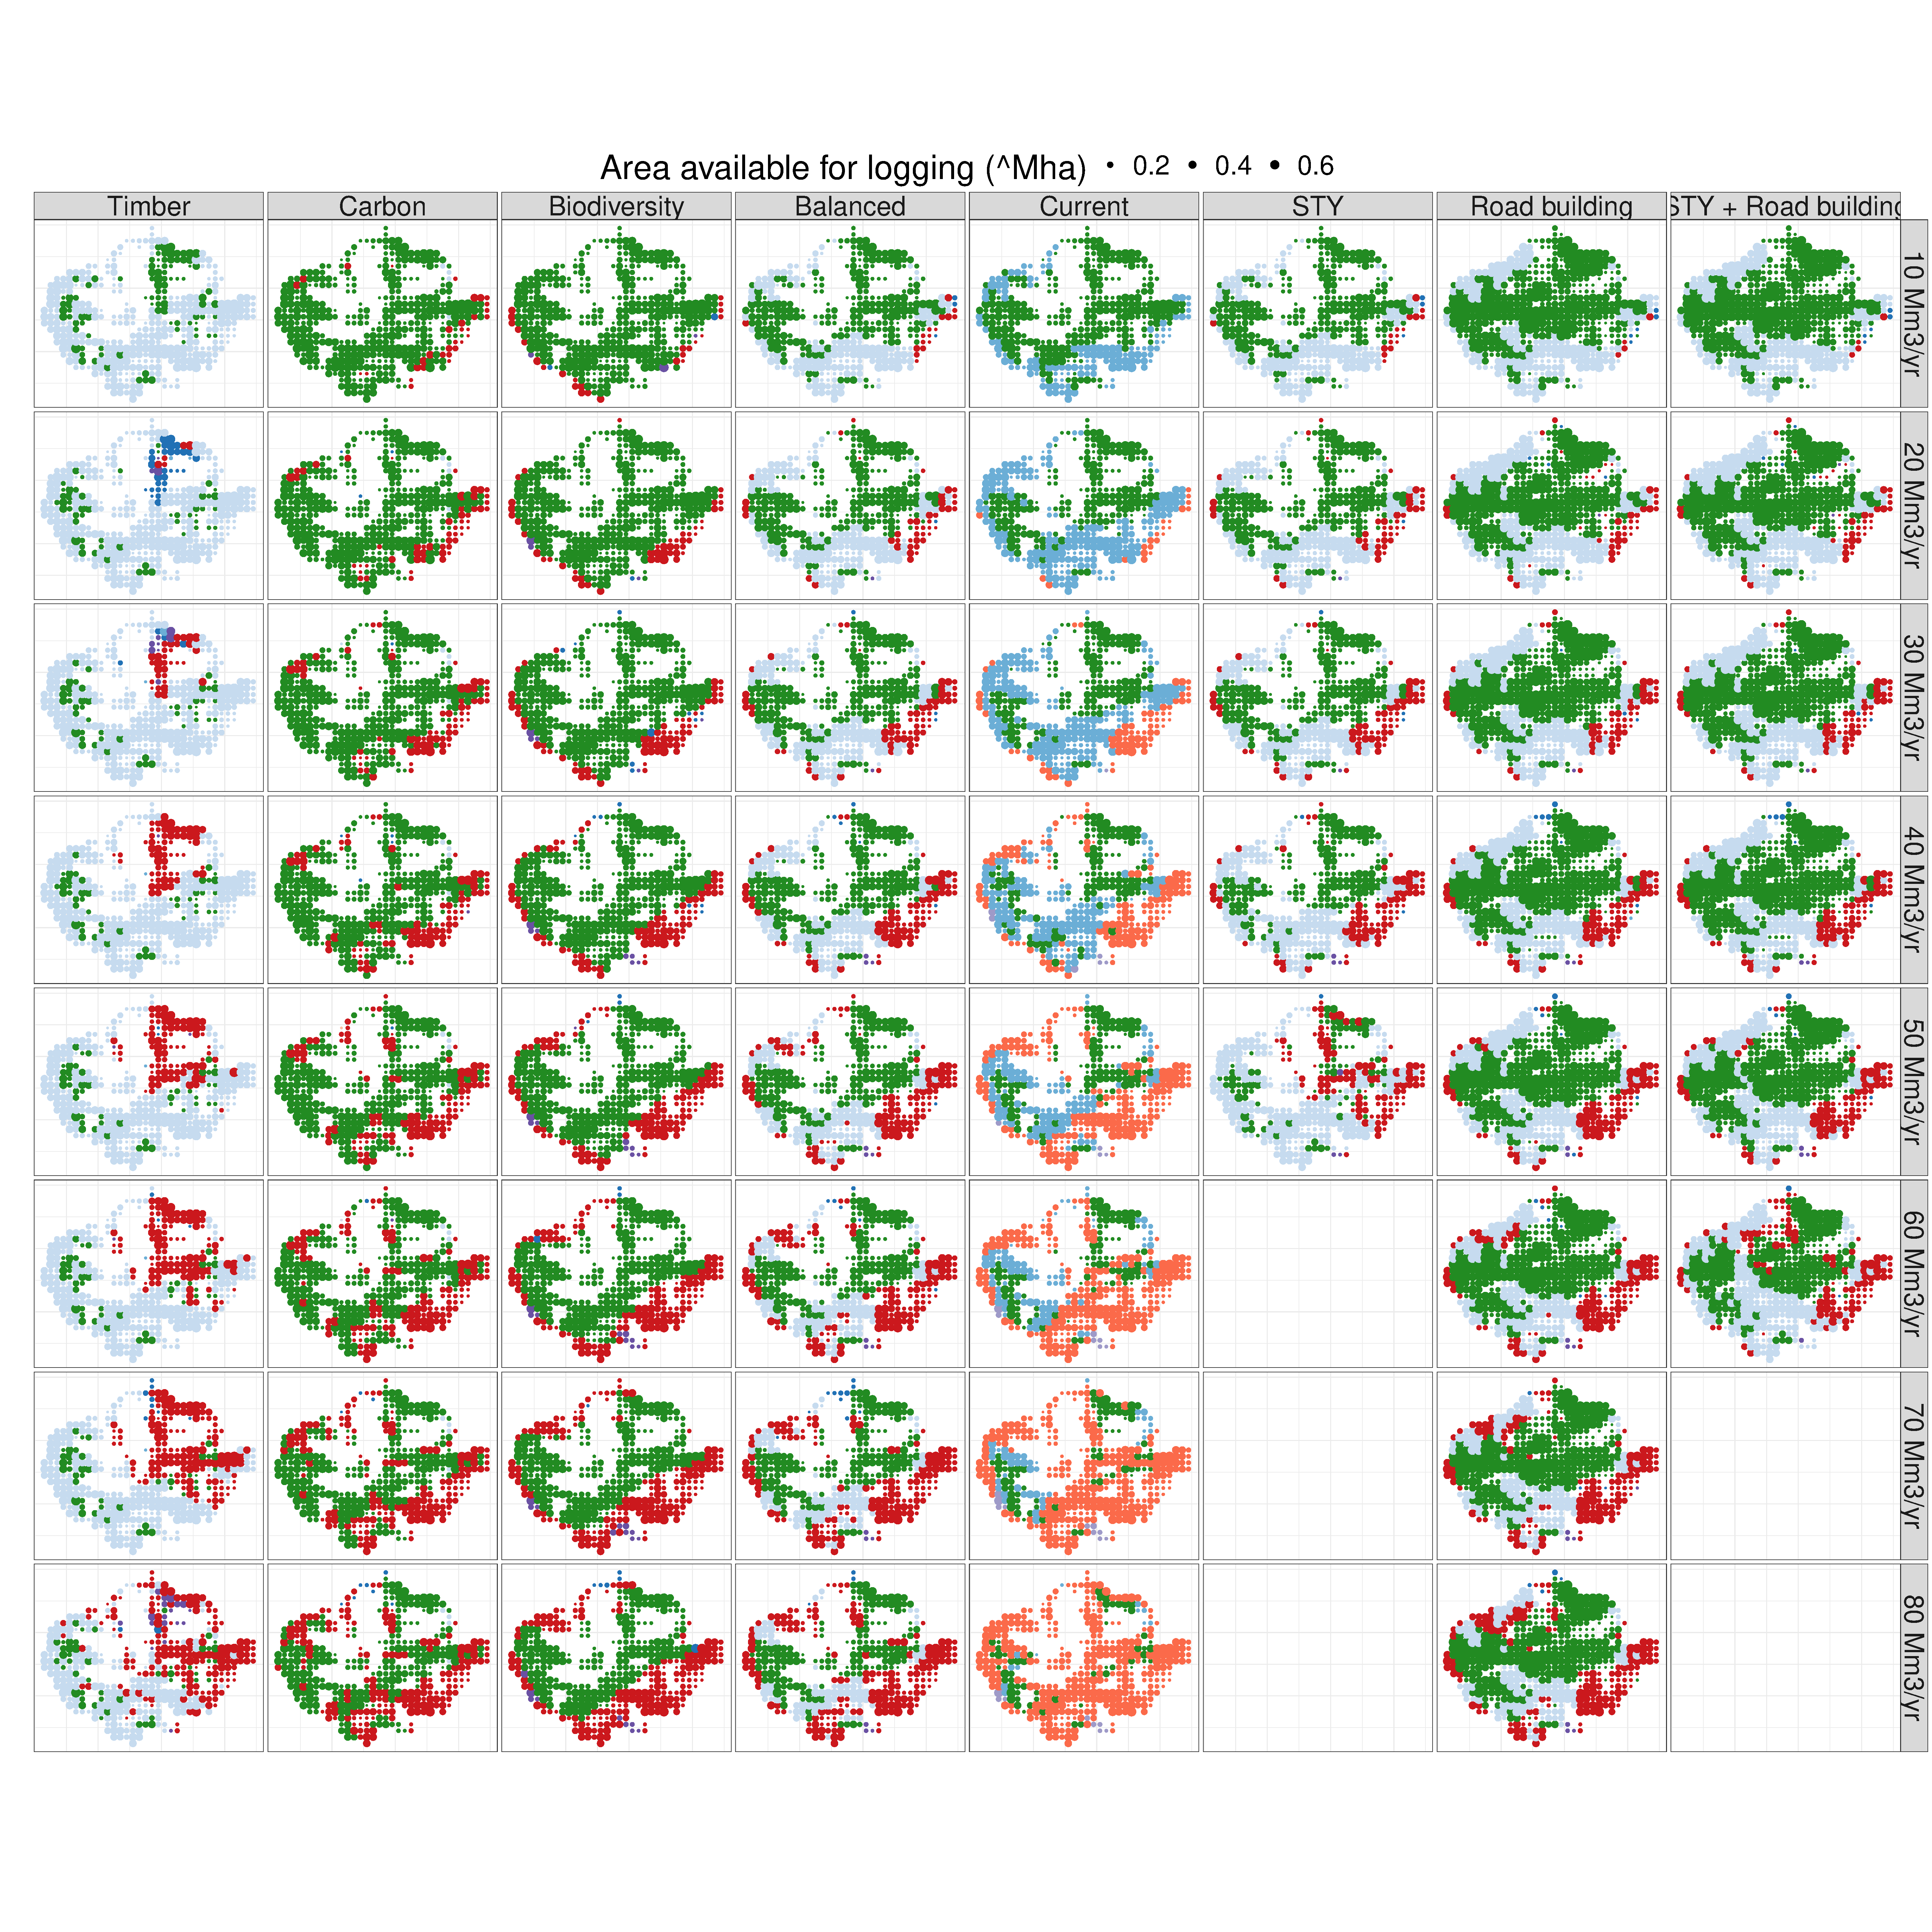
\includegraphics[width=\linewidth]{graphs/mapsChangeDemand.pdf}
    \caption{Results of spatial optimisation with varying demand for timber (from 10 to 80 Mm$^3$/yr), and under different scenarios.}
    \label{fig:mapsIncDemand}
\end{figure*}

\end{document}